%Git-rapport
\documentclass[a4paper]{article}

\usepackage[swedish]{babel}
\usepackage[utf8]{inputenc}
\usepackage{graphicx}
\setcounter{secnumdepth}{4}
\usepackage{titlesec}
\usepackage{caption}
\usepackage{float}
%For figures
\graphicspath{ {Figures/} }
\captionsetup{justification=centering}

\begin{document}

\begin{titlepage}
\centering
{\bfseries\huge Projektrapport DAT290}

\vspace{10mm}

{\Large Radiostyrd Bil, Grupp 07}

\vspace{20mm}

{\Large \itshape{Anders Berggren Sjöblom, Johanna Gudmandsen, Gustav Holst, Joakim Junttila, Henrik Klein Moberg, Carl Lundgren, Stanisław Zwierzchowski}}

\vspace{10mm}

%Vet ej vilket datum som ska stå
{DATUM}


\normalsize{
\begin{table}[b]
\centering
\begin{tabular}{|l|l|l|}  \hline
         & \bf Namn & \bf Datum   \\ \hline \hline
Granskad & NAMN     & DATUM        \\ \hline
Godkänd  & NAMN     & DATUM         \\ \hline
\end{tabular} 
\end{table}}
\end{titlepage}

\tableofcontents

\newpage
\noindent {\Large \bf Ordlista}


\vspace{5mm} \noindent
{\bf ADC} - Analog to digital converter, översätter analoga värden i enheten Volt till digitala värden~\cite{ADC}.

\vspace{5mm} \noindent
{\bf ARM} - En processorarkitektur~\cite{chalmersARM}.

\vspace{5mm} \noindent
{\bf Avståndsmätare} - Mäter avstånd från ett objekt med hjälp av ultraljud och dess eko~\cite{DistMeasure}. Modul som används i detta projekt är HC-SR04.

\vspace{5mm} \noindent
{\bf Bluetooth-moduler} - Är antingen sändare eller mottagare och möjliggör för radiofrekvensiell överföring genom parning mellan moduler~\cite{Bluetooth}. Modul som används i detta projekt är HC-05.

\vspace{5mm} \noindent
{\bf GPIO} - General-purpose input/output~\cite{chalmersARM}.

\vspace{5mm} \noindent
{\bf Oscilloskop} - Instrument som används till att mäta elektriska signaler under en viss tid~\cite{oscilloscope}.

\vspace{5mm} \noindent
{\bf Potentiometer} - En elektrisk komponent som med hjälp av ett variabelt motstånd kan begränsa spänning~\cite{Potentiometer}.


\vspace{5mm} \noindent
{\bf PWM-signaler} - PWM eller Pulse Width Modulation är en moduleringsteknik som mest används för att styra mängden elektrisk ström som förs till exempelvis en motor~\cite{PWM}.

\vspace{5mm} \noindent
{\bf RF-moduler} - Radiofrekvensmoduler. Är antingen sändare eller mottagare och möjliggör för radiofrekvensiell överföring~\cite{RFModule}.

\vspace{5mm} \noindent
{\bf UART} - Universal Asynchronous Receiver/Transmitter~\cite{chalmersARM}.

\vspace{5mm} \noindent
{\bf USART} - Universal Synchronous/Asynchronous Receiver/Transmitter~\cite{chalmersARM}.





\newpage
\section{Introduktion}

%Radiostyrda bilar började produceras på mitten av 60-talet~\cite{RCHistory}. De första radiobilarna drevs med hjälp av bensin och hade grova däck då de skulle köras utomhus. Det var inte förrän 1974 motorerna ersatter av elektriska och kort därefter startade tävlingar med dessa bilar. Detta eskalerade och radiobilen nåde extrem popularitet under 80-talet. Då kom även fler tävlingar och bilarna utvecklades för att kunna köra snabbare.

Radiostyrda bilar började produceras på mitten av 60-talet~\cite{RCHistory}. De första radiobilarna drevs med hjälp av bensin och körde relativt långsamt. Ett drygt decennium senare ersattes motorerna med elektriska varianter och kort därefter började tävlingar hållas. Detta ledde till en väldig popularitet för radiobilen som hobby och utvecklingen av den lade stor vikt vid snabbhet. Trots dessa mindre justeringar har den radiostyrda bilens uppbyggnad i det stora hela förblivit densamma.

\subsection{Syfte}

Syftet med detta projekt är att uppdatera den klassiska radiostyrda bilen genom att ersätta befintlig sändare samt mottagare i en radiostyrd bil med nya datorer och även möjliggöra styrning från en Androidtelefon. Avsikten är även att implementera en kontrollapplikation som ska kunna stoppa bilen från att kollidera. Följden av detta blir en produkt mer anpassad till aktuell teknik och det erhålls på så sätt en mer modern teknisk produkt.


%Syftet med detta projekt är att uppdatera den klassiska radiostyrda bilen med hjälp av ny teknik som bluetooth. För att följaktligen erhålla en mer modern teknisk produkt.

\subsection{Mål}
Projektets övergripande syfte bryts upp i delmål som mer detaljerade är angivna nedan.

\begin{itemize}
\item Den befintliga sändaren samt mottagaren som finns i handkontrollen respektive bilens elektronik byts ut mot ARM-baserade system (se Figur 1). Dessa ska vid färdig produkt kontrolleras via Bluetooth.
\item En kontrollapplikation implementeras. Med hjälp av en avståndsmätare är avsikten att bilen ska kunna köra rakt fram i högsta möjliga hastighet där bilen på ett avstånd av 1 cm från ett objekt självständigt kan bromsa in utan att kollidera. Kontrollapplikationen kan aktiveras från samtliga sändare.
\item Styrning via mobilapplikation realiseras. Bilen kan manövreras genom ett Andriodsystem via Bluetooth.
\end{itemize}

\begin{figure}[H]
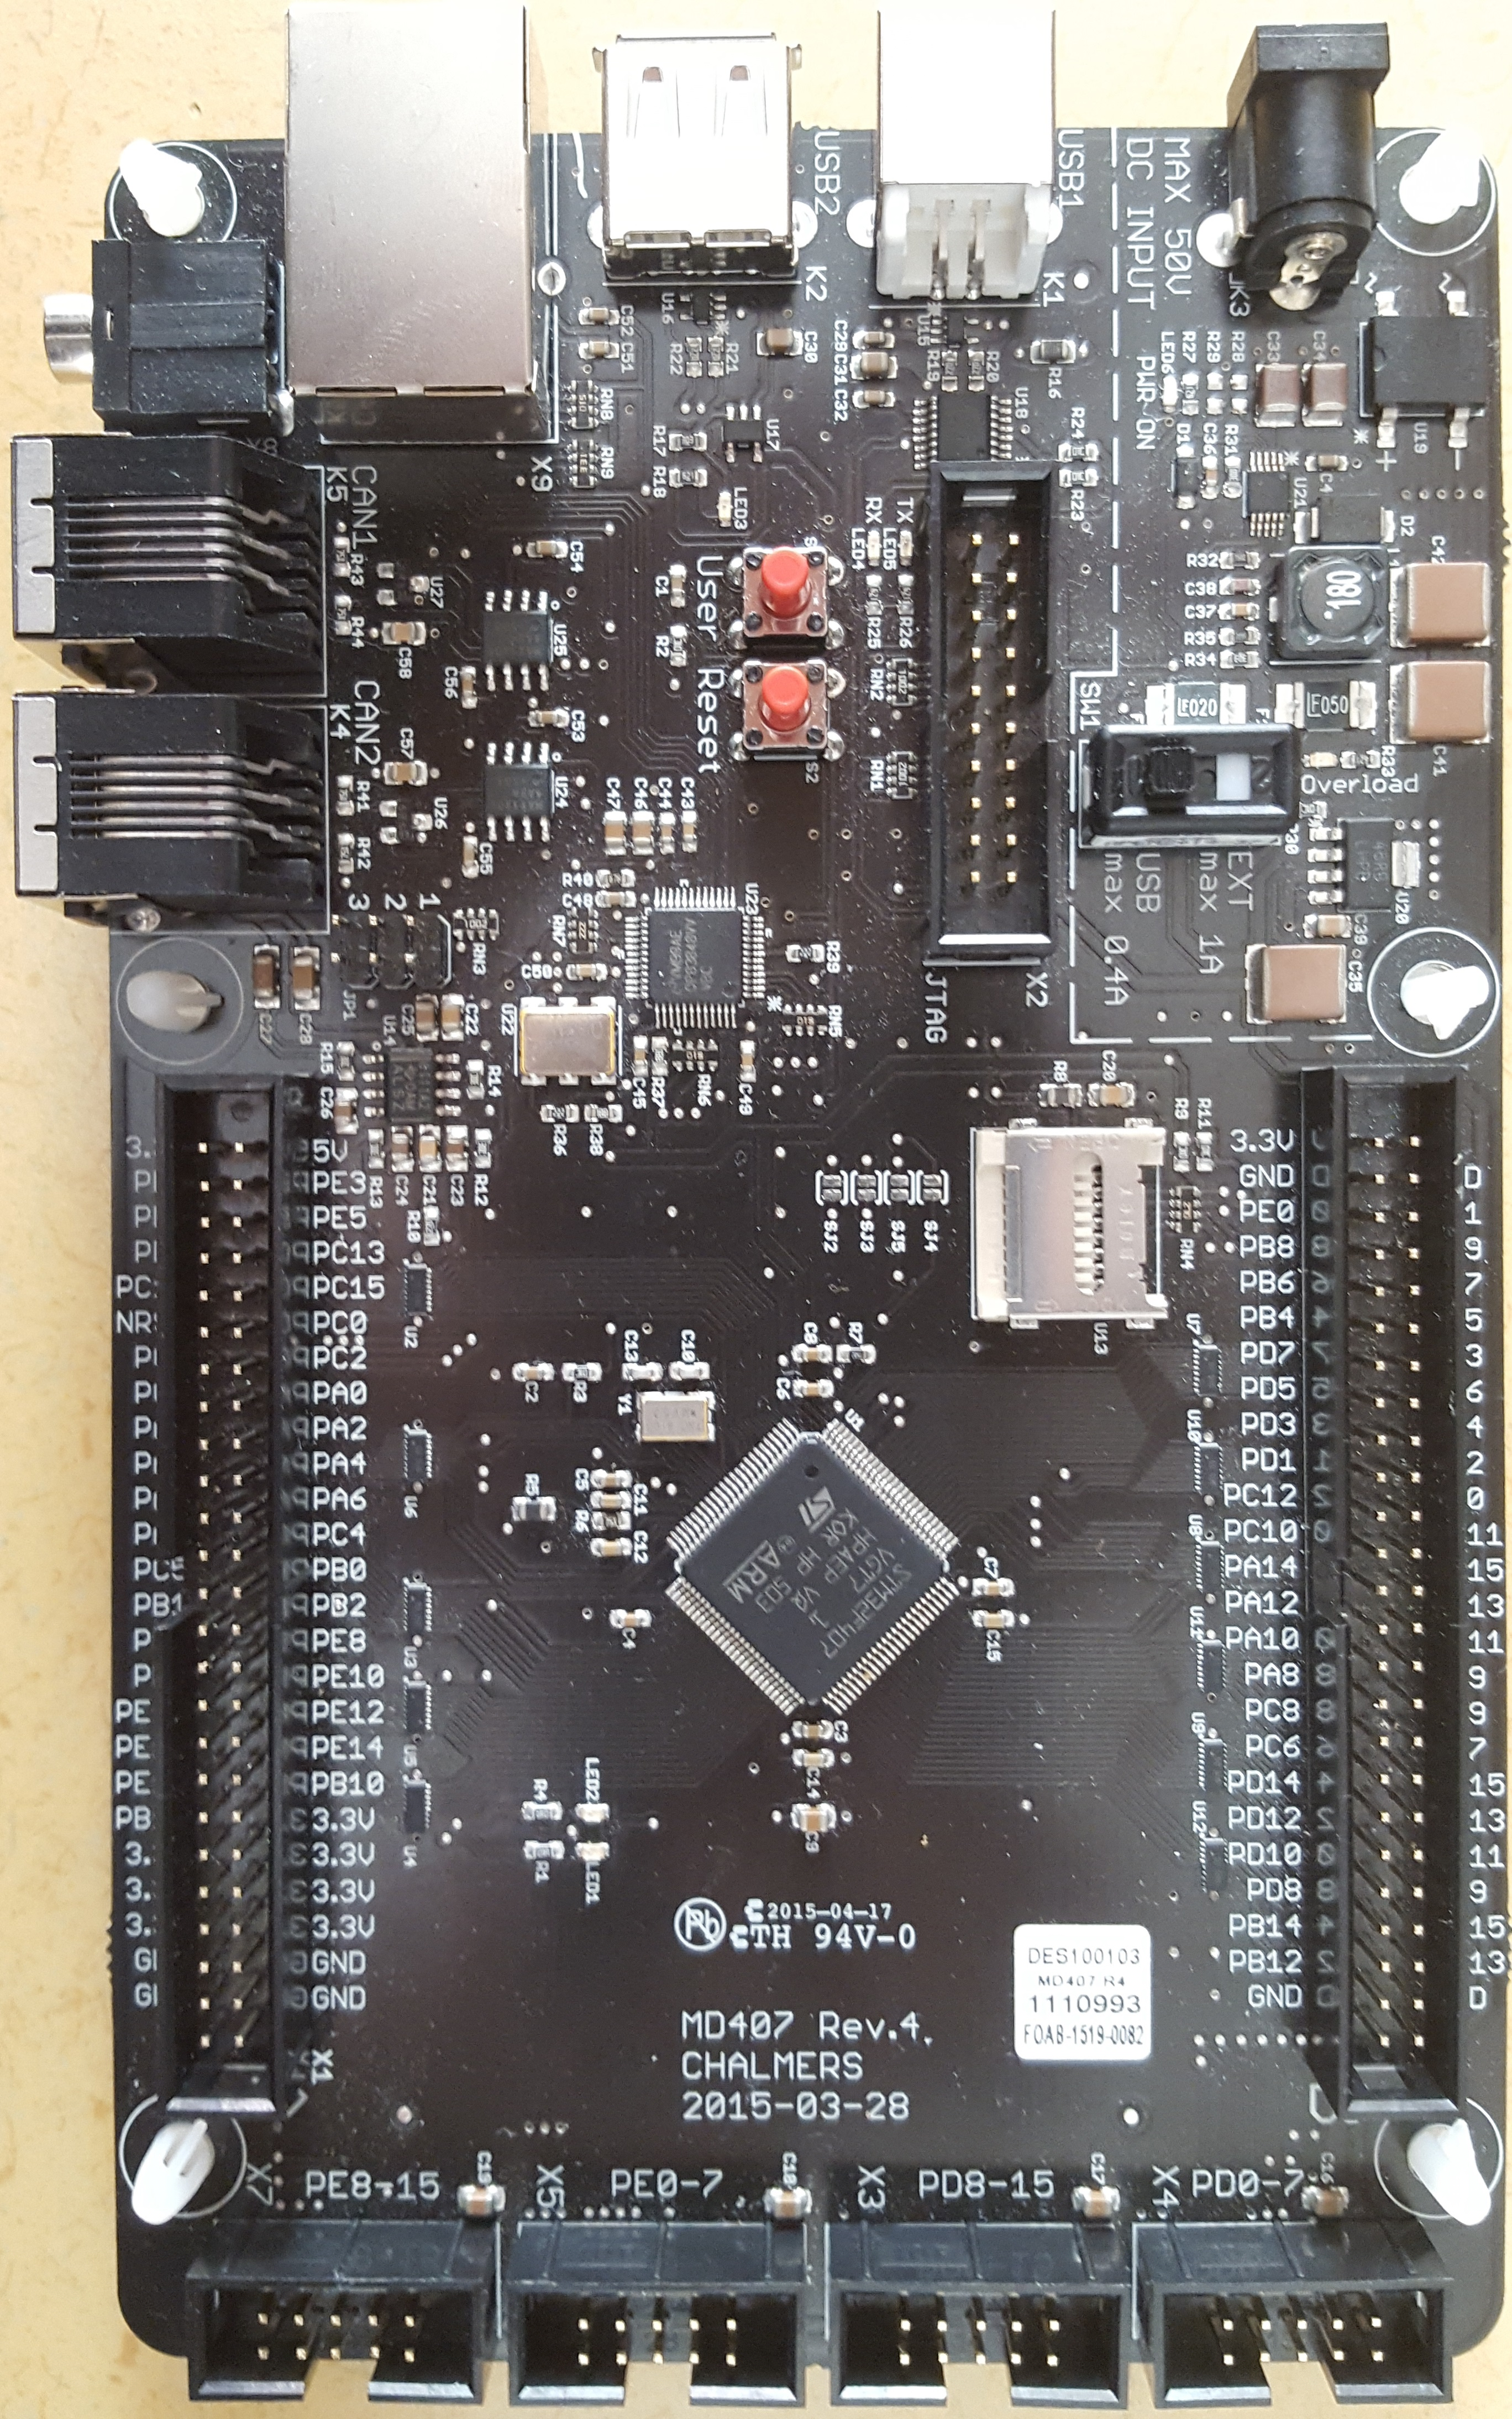
\includegraphics[scale=0.03]{MD407.jpg} \hspace{2mm}
\centering
\caption{\it MD407, en ARM-dator.}
\end{figure} 

%Målförslag
%Projektet går ut på att ersätta delar av elektroniken i en radiostyrd bil. Sändaren samt mottagaren som finns i handkontrollen ska bytas ut till en ny handkontroll. Nya handkontrollens sändnings singnal kommer ändras till att slutligen bli  Bluetooth. I samband med singnal bytet kommer nya handkontrollen att anpassad till andara ändringar som ska genomföras. Andra ändringar som ker berör bland annat skälva bilen. Bilens elektronik ska bytas ut mot ARM-baserade system. Vidare ska en kontrollapplikation implementeras i bilen med hjälp av ett antal avståndsmätare. Därefter ska bilen programeras så den självständigt ska kunna köra rakt fram i högsta möjliga takt och bromsa in helt på ett avstånd av maximalt 1 cm från en vägg. Sista steget i arbetsprosessen är att med hjälp av Bluetooth signalen utveckla en aplickation som ska kunna styra bilen och fungera som en fullfjädrad handkontroll.

\subsection{Arbetsmetod}
I detta avsnitt finns en överblick av hur projektet utförts vid olika moment. Det börjar med ett avsnitt över projektets administration och följs av en beskrivning av varje komponent som konstrueras i systemet. Dessa är angivna i ordningen de utförs.

\subsubsection{Allmänt: Projektledning}
Dokumentation och kommunikation utförs enligt planen för projektet. Ett versionshanteringssystem, Git, används för att enkelt kunna lagra filer mellan olika datorer. Applikationen Slack utnyttjas för att möjliggöra för strukturerad kommunikation och utöver detta sker möten en gång i veckan för att varje projektgruppsmedlem ska få aktuell information. Veckovisa meddelanden för projektets fortskridande har givits till uppdragsgivaren, detta på grund av att det ska vara enkelt att följa utvecklingen. Projekgruppen delades upp i mindre grupper där de självständigt fokuserade på första och andra målet, tredje målet, och dokumentationen.

\subsubsection{Allmänt: Kodning}
Standarder för kodning är bestämd för underlätta implementation. Programkoder är för samtliga komponenter förutom Androidapplikationen skrivna i C med utvecklingsmiljön Codelite. Utvecklingen av applikationen skedde istället i Java genom Eclipse och importerades sedan till Andriod Studio, en miljö där stöd för att skapa Androidapplikationer finns. För att kunna överföra kod till datorenheterna som ersätter mottagare och sändare utnyttjas programmet ETERM. En kompilerad kod exekveras då och genom direktkoppling till en port på respektive enhet kan koden sparas och senare användas. Hjälpfunktioner till all programkod har erhållts från datorenheternas egna programbibliotek samt STMicroelectronics. 

%en utvecklingsmijö för Andriodapplikationer - ORDLISTA

\subsubsection{Delsystem: Konstruktion av mottagare}
Projektet inleds med att mäta upp befintliga styrsignaler. För att kunna återskapa signalerna som skickas från den ursprungliga mottagaren till bilens styrelektronik mättes signalerna upp med hjälp av ett oscilloskop. Det som möjliggjorde detta var ett tillhandahållet kretskort som kopplat till bilens kontrollenhet kunde separera signalerna. Bilens samtliga funktioner testades och utslagen blev de värden som användes till verifiering för korrekt replikering av styrsignaler. Signalerna är av typen PWM och både dess cykeltid och frekvens mättes upp i motorns och rattutslagens maximala lägen. 

\vspace{5mm} \noindent
Den nya mottagaren återskapar dessa signaler. En MD407-enhet ersätter den ursprungliga mottagaren och dess systemklocka utnyttjas för att skicka rätt styrsignaler till korrekt styrelektronik. Dessa värden testas utförligt för att kunna säkerställa att de replikerande styrsignalerna är identiska i jämförelse med de ursprungliga.


%Mottagaren ersätts med en ny datorenhet, MD407. Denna erhåller seriellt bytes som skickas från en sändare (se Figur 2). Byten analyseras och dess systemtimer utnyttjas för skicka rätt signal till korrekt styrelektronik.

%Enheten MD407 användes och dess systemtimer utnyttjades för att möjliggöra för att rätt signal skickas till rätt del i styrelektroniken. När mottagaren seriellt erhåller värden är detta via bytes (se Figur 2). Dessa analyseras i datorenheten 

%kopplas ett kretskort, Adapter Maverick, till bilens egna kontrollenhet, MRX-242. Kretskortet har möjlighet att separera mottagarens signaler och kopplat till ett oscilloskop går det att urskilja specifika signaler så de tydligt kan mätas upp. Intervall för frekvens och cykeltid identifierades och specfierades enligt motorns och rattutslagens olika lägen.

%Signalerna är av typen PWM och deras värde bestäms av medelspänningen. 


%\subsubsection{Konfiguration av ny mottagare}
%Mottagaren i bilen ersätts först med en ny datorenhet. Enheten MD407 används här för att byta ut den ursprungliga mottagaren. Systemets integrerade klocka användes för att replikera de ursprungliga signalerna som tidigare mätts upp. Med hjälp a pulsbredsmodulering kunde dessa


%En MD407-enhet ersätter mottagaren i bilen. På enheten finns ett integrerat kretskort som hanterar systemets timer. Denna konfigureras till att hantera utdatan som direkt är kopplad till bilens styrelektronik. 
%
%Information erhålls en mottagande modul. Mottagaren tar seriellt emot bytes 

%En MD407-enhet ersätter mottagaren i bilen. Kanalerna CH3 och CH4 på det integrerade timer-kretskortet, TIM2, konfigureras för att hanteras av portarna PA2 respektive PA3 i C-koden. Koden, utvecklad i Codelite, initierar CH3 till att reglera motorstyrningen och CH4 till att kontrollera rattutslagen. Följden av detta blir att portarna PA2 och PA3 i den ersättande mottagaren kopplas direkt till bilens styrelektronik, en kabel till motorn och en till styrservot. 

%\vspace{5mm} \noindent
%Information tas emot genom en mottagande modul. När mottagarmodulen erhåller ett meddelande triggas en funktion i koden. Denna ska undersöka vilket kommando som ska utföras samt till vilken grad detta skall göras enligt bitarnas anvisningar i Figur 2. Värdet 1 eller 2 på kommandobitarna leder till att bilens motor eller styrservo påverkas i angiven ordning. Tar mottagaren exempelvis emot kommandot att bilen ska ändra motorhastigheten skickas denna information till motorns styrelektronik. Den nya hastigheten beror på storleken av värdet. Värdet på meddelandet från sändaren skickas som en PWM-signal till den begärda styrelektroniken i bilen som fångar upp dessa under en period(se exempel i Figur 3), uppfattar värdet och agerar. Detta arbete har förenklats med hjälp av kodbibliotek från STMicroelectronics som innehåller funktioner för att initiera PWM-genererande. Observera att bilen endast svarar korrekt på värden där PWM-signalen är hög under ungefär 8\%-12.4\% av perioden, en högre eller lägre andel än detta kan få elektroniken att överbelastas. Värden i meddelanden mellan RF-modulerna kan antas från 0-63, utifrån 6 bitar, och TIM2 konfigureras därför till att addera en offset av 110 innan PWM-signalen skickas till styrelektroniken för att möjliggöra för korrekt avläsning.

%\begin{figure}[H]
%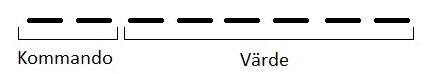
\includegraphics[scale=1]{aByteComVal.jpg}
%\centering
%\caption{\it Specifikationer av byten som seriellt skickas från sändare till mottagare.}
%\end{figure} 

%\begin{figure}[H]
%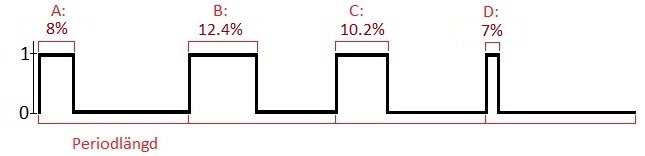
\includegraphics[scale=1]{PWMsignals.jpg}
%\centering
%\caption{\it Exempel på möjliga PWM-signaler. Om byten indikerar att motorn ska påverkas kommer den i fall A och B köra i högsta fart baklänges respektive framlänges. I fall C hamnar bilen i neutralt läge och står då stilla. Signalen i fall D tolkas ej av bilens styrelektronik då det ligger utanför dess avläsningsintervall.}
%\end{figure} 


\subsubsection{Delsystem: Konstruktion av sändare}
En datorenhet, MD407, ersätter sändaren. Reglage för styrning implementas med hjälp av en potentiometer (se Figur XX), vilken kopplas till datorenheten. Värdena datorenheten erhåller från potentiometern översätts från analoga till digitala genom en integrerad ADC. Detta implementeras med hjälp av stödfunktioner från de tidigare nämnda kodbiblioteken.

\begin{figure}[H]
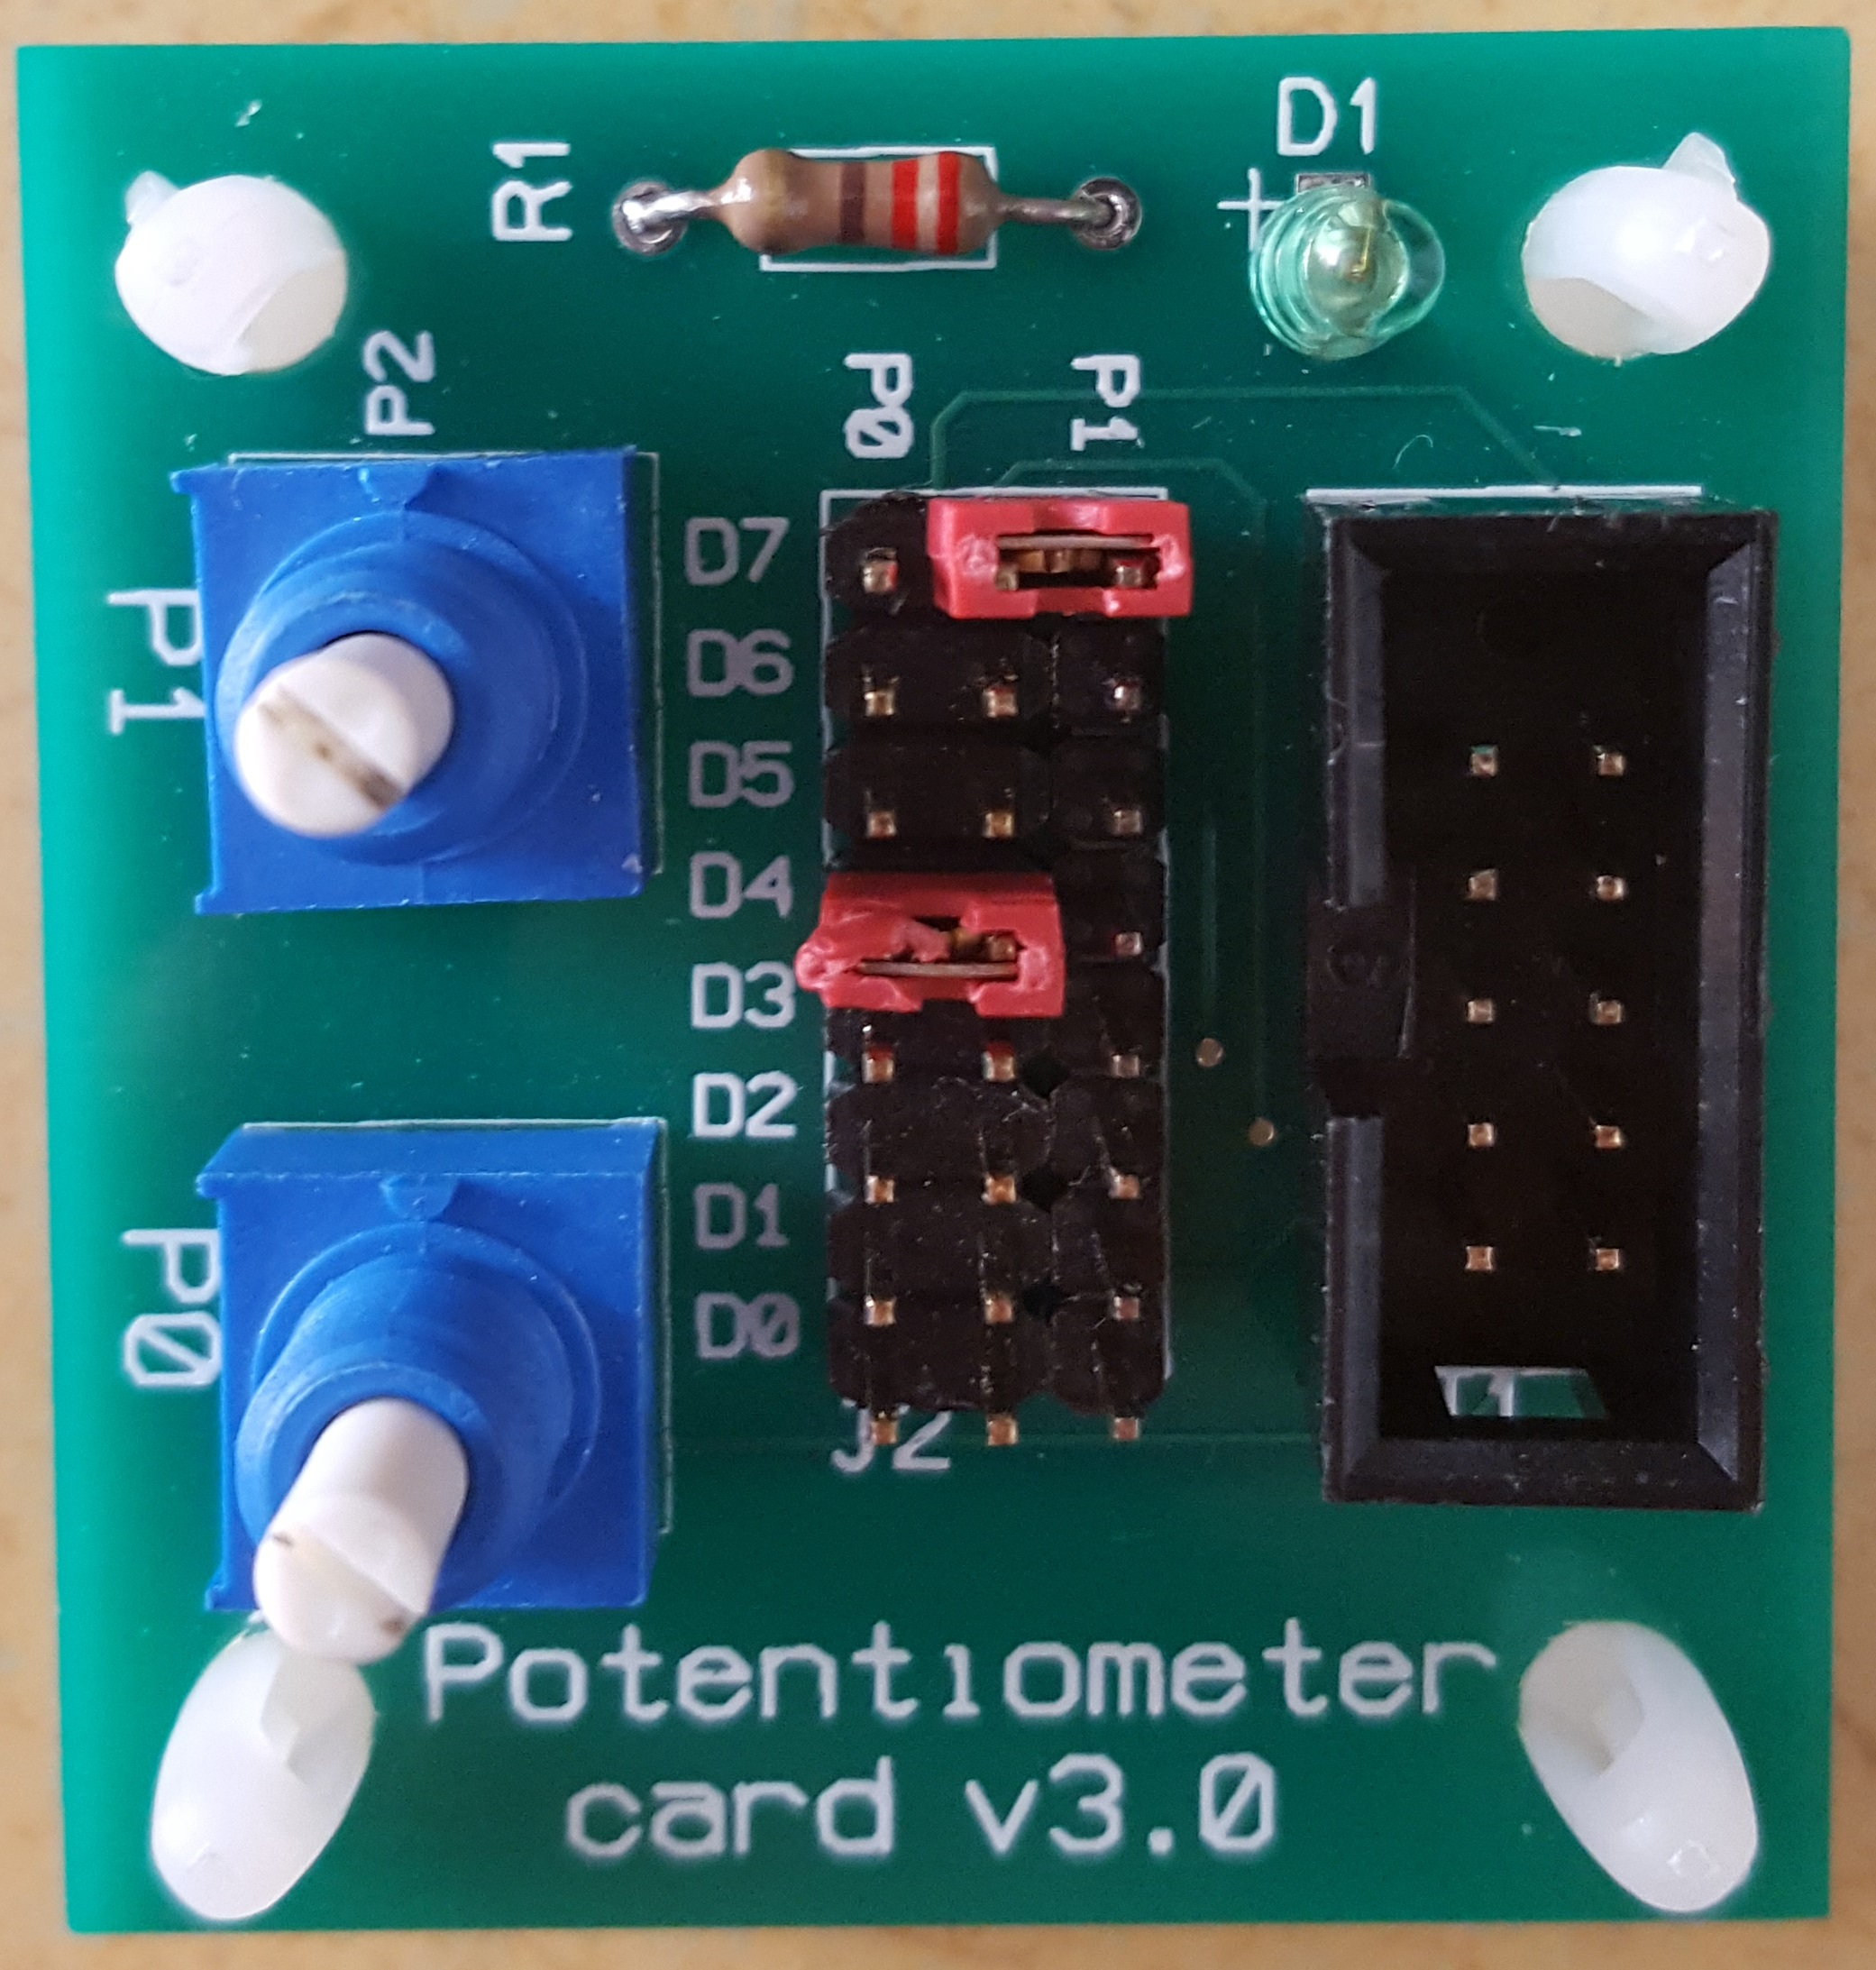
\includegraphics[scale=0.04]{Potentiometer.jpg}
\centering
\caption{\it En potentiometer.}
\end{figure} 



%\begin{figure}[H]
%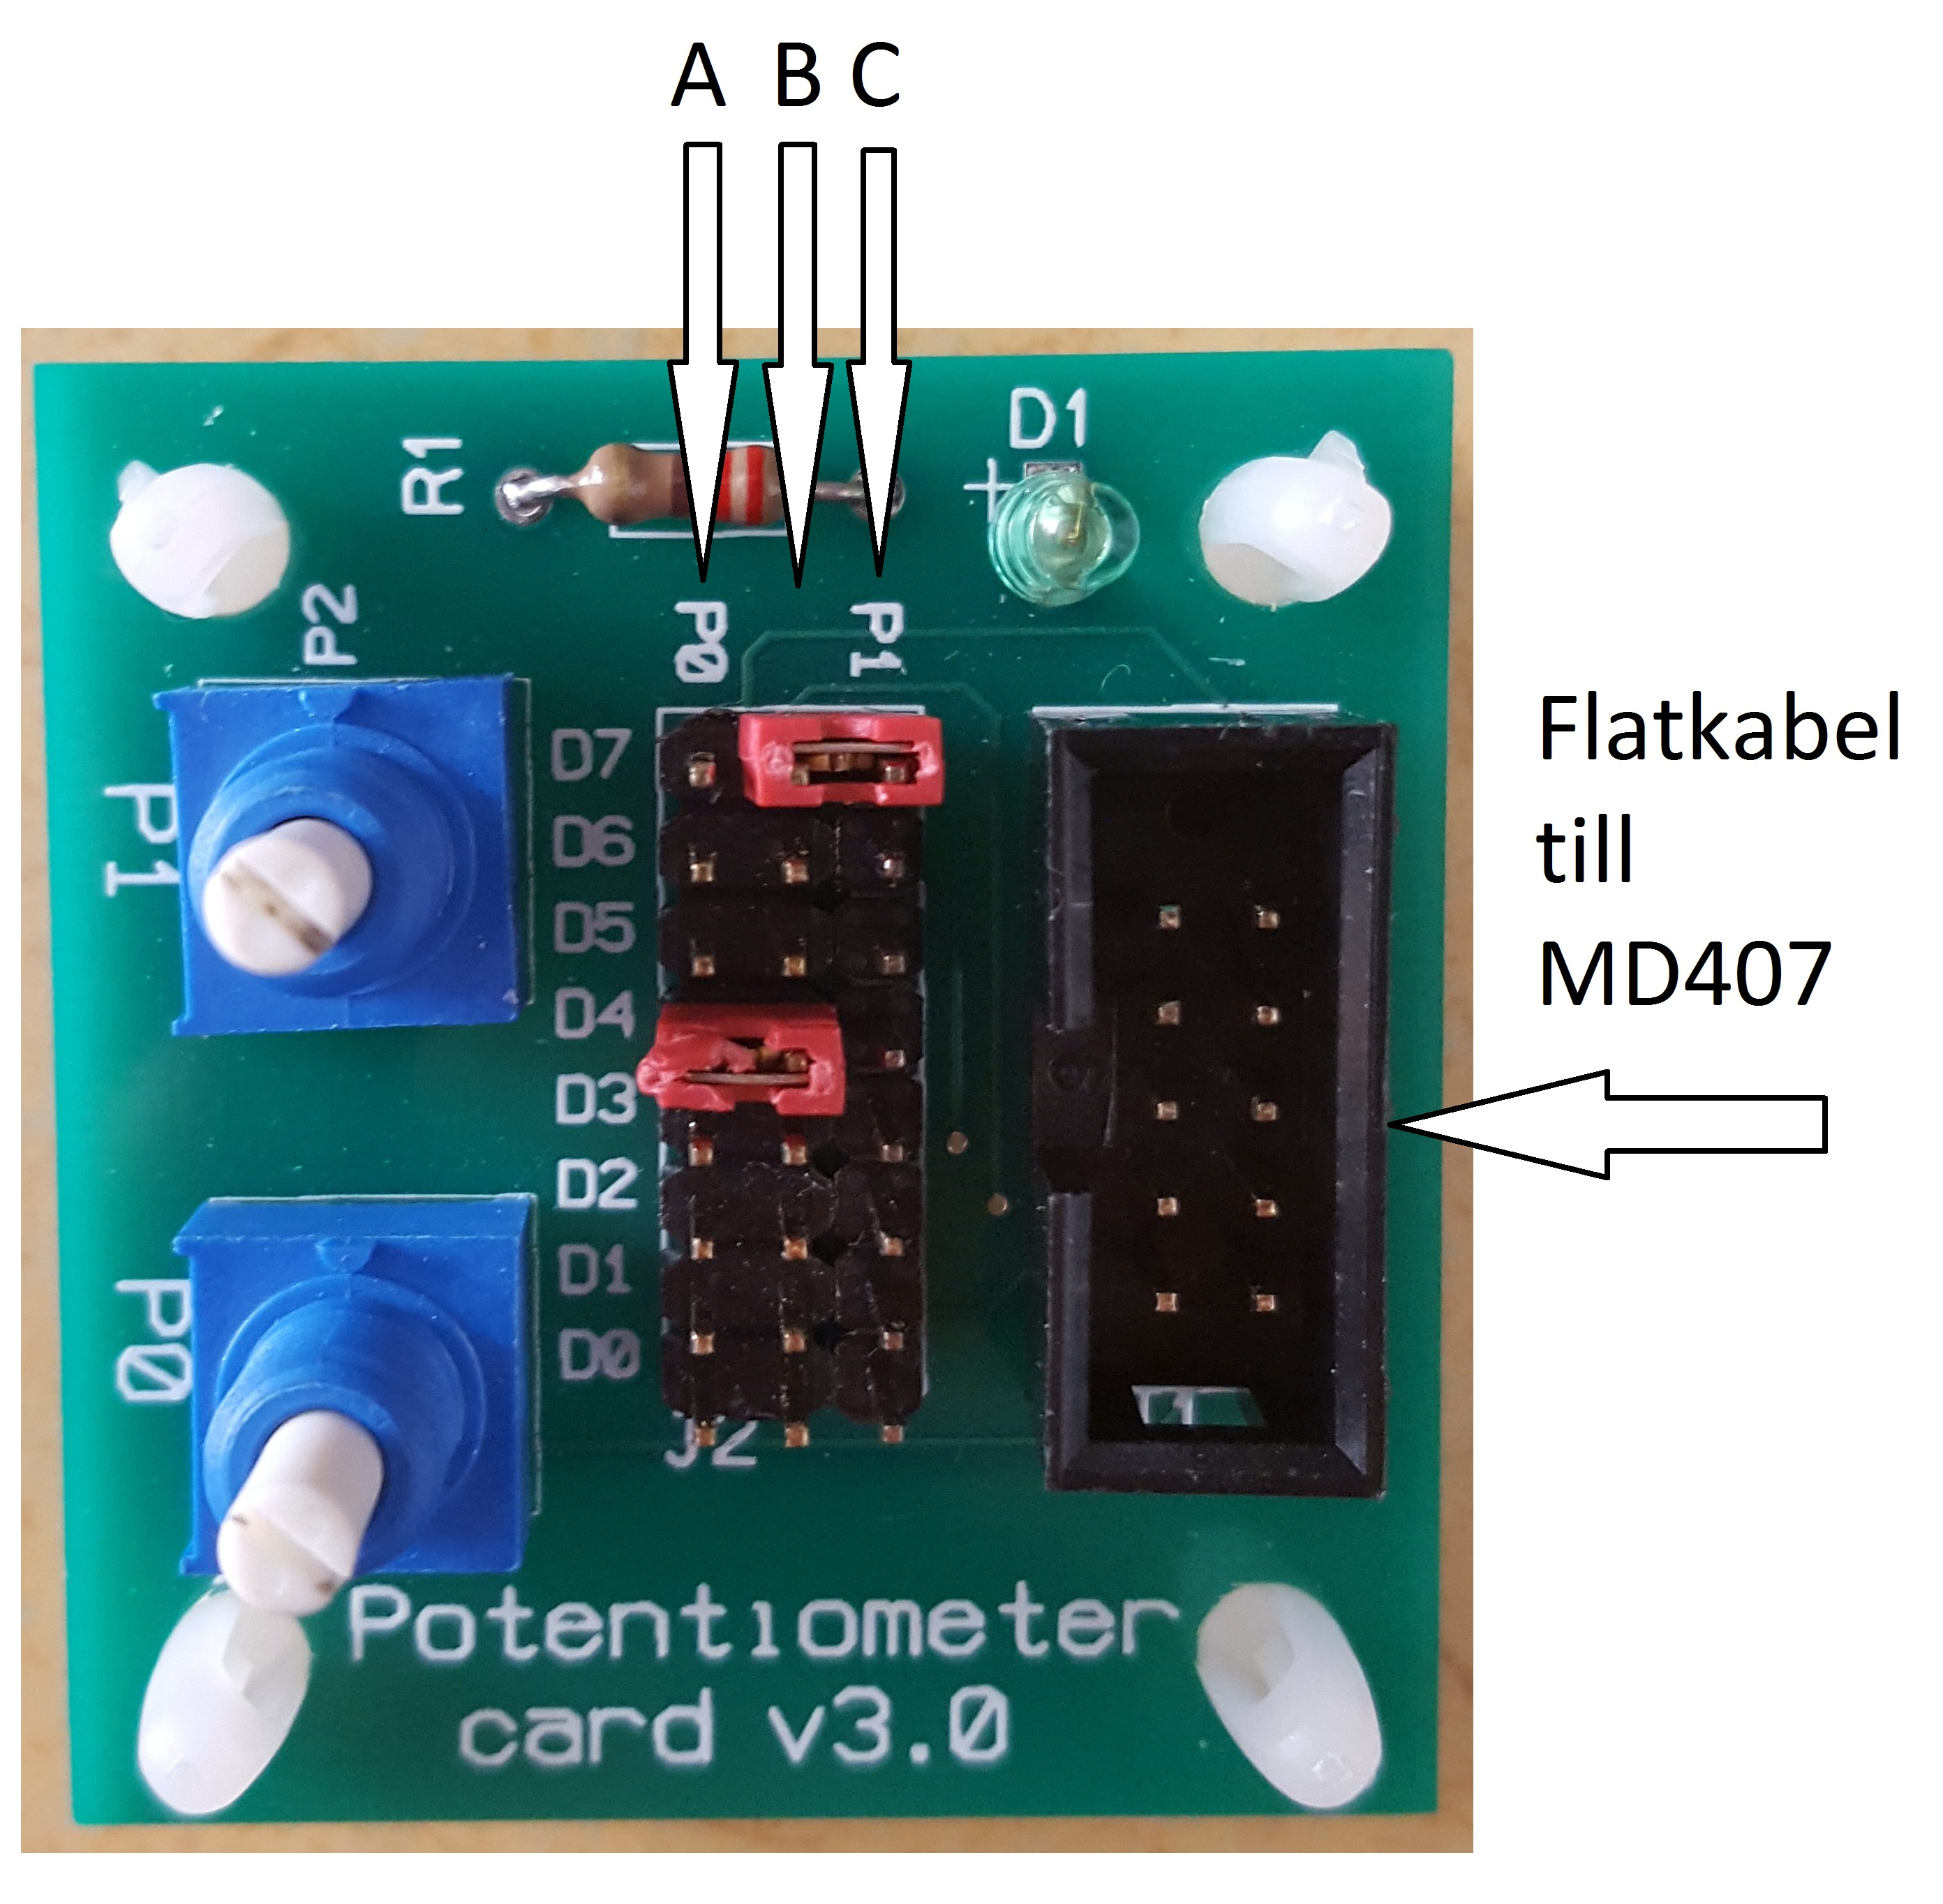
\includegraphics[scale=0.05]{PotentiometerMedRitning.jpg}
%\centering
%\caption{\it En potentiometer. A, B och C representerar kolumner. B leder ström och kopplas till A respektive C med kort kabel såsom bilden visar. För att få värden till datorenheten kopplas även en kabel från A, rad 1, och C, rad 4, till MD407}
%\end{figure} 

\subsubsection{Delsystem: Radiolänk mellan mottagare och sändare}
Datorenheterna kommunicerar via en radiolänk. Primärt kopplas en RF-mottagare och en RF-sändare (se Figur XX) på respektive enhet för att möjliggöra för ett informationflöde över 433MHz-bandet. När systemet fungerar med med dessa ersätts de av Bluetooth-moduler (se Figur XX) som istället kommunicerar över en frekvens av 2.4GHz. Kommunikation över Bluetooth kräver initiering av roller till modulerna vilket görs genom AT-kommandon. 



\begin{figure}[H]
\centering
\includegraphics[scale=0.06]{RF-transmitter.jpg}
\includegraphics[scale=0.05]{RF-receiver.jpg} \\ \vspace{2mm}
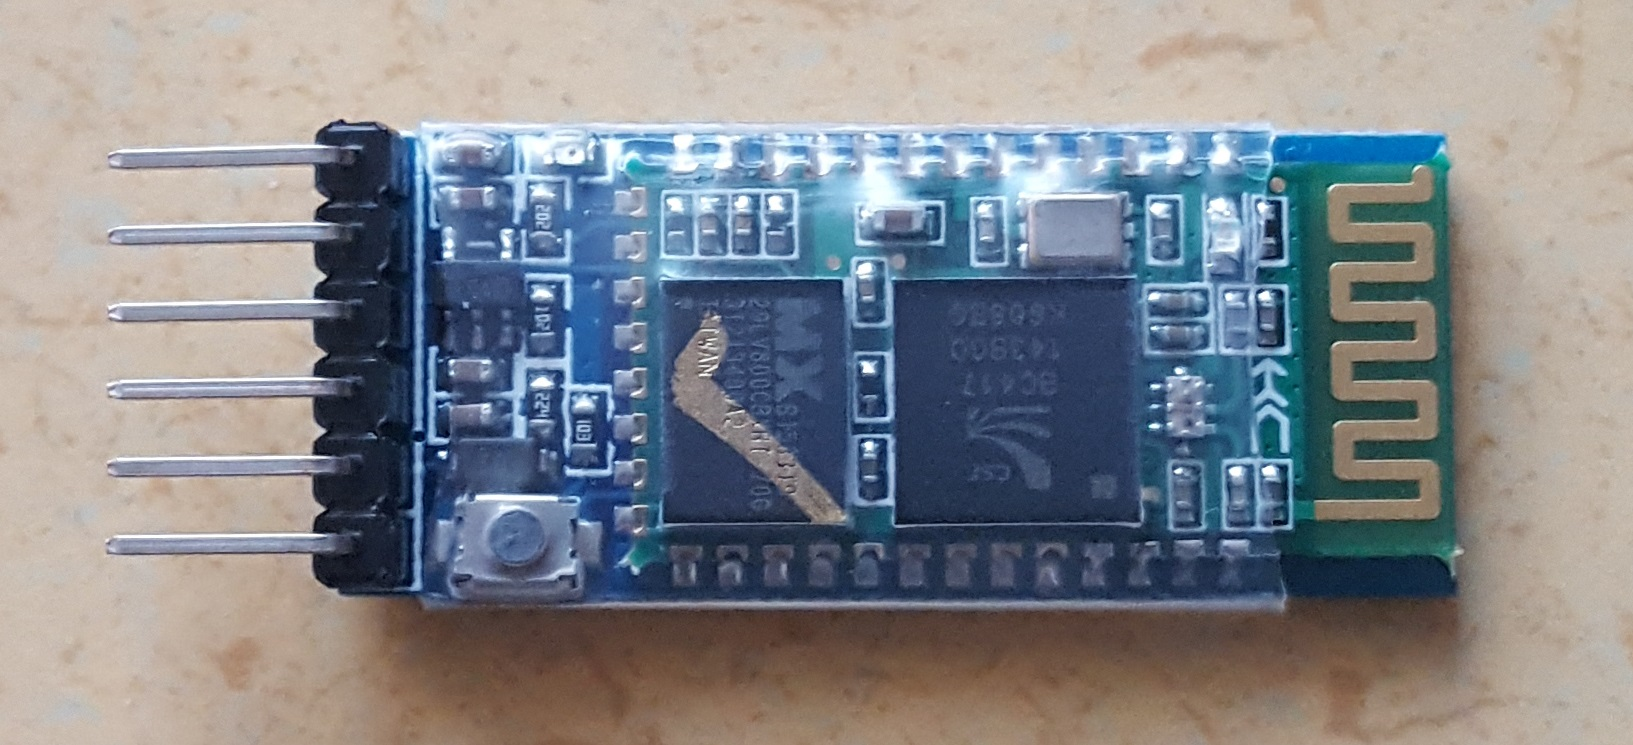
\includegraphics[scale=0.07]{BluetoothFront.jpg}
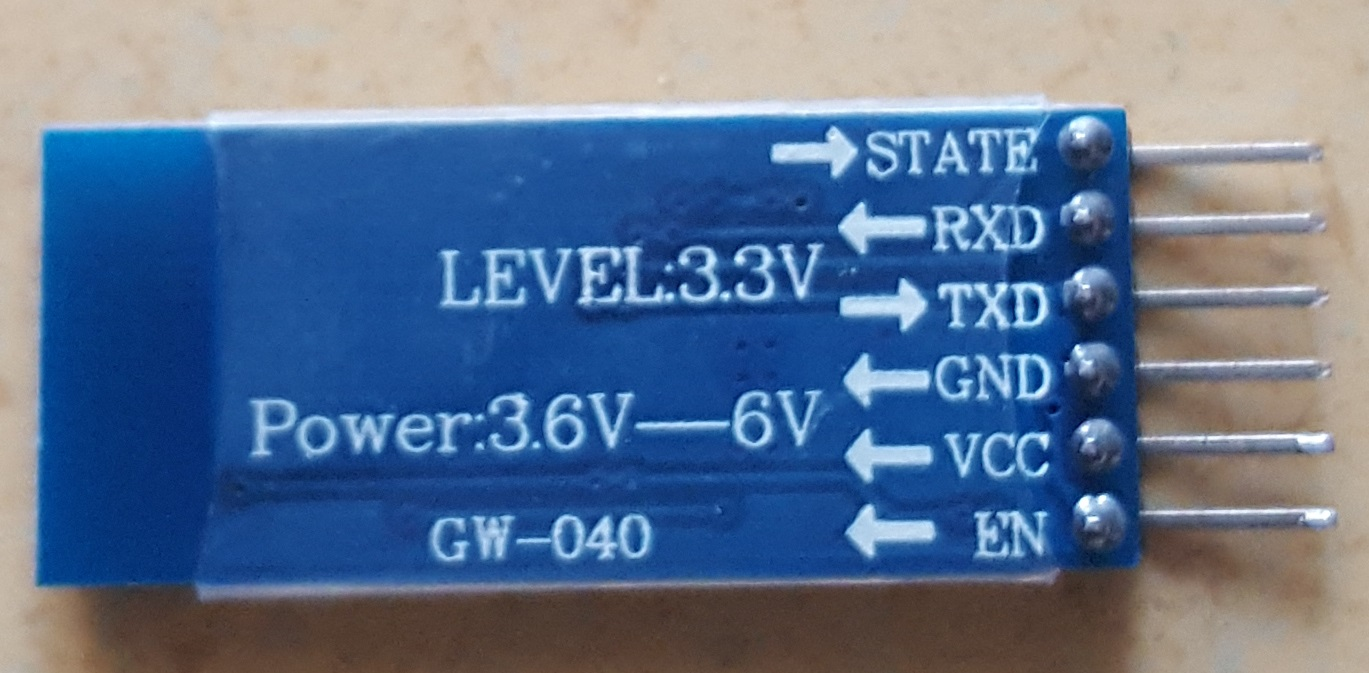
\includegraphics[scale=0.078]{BluetoothBack.jpg}

\caption{\it På övre raden ses en RF-mottagare samt RF-sändare (i angiven ordning) och på undre raden en Bluetooth-moduls framsida samt baksida (i angiven ordning)}
\end{figure} 




\vspace{5mm} \noindent
Radiolänken verifieras kontinuerligt. Mottagar- och sändarmodul kopplas om vid varje tillfälle för att erhålla det konstanta flödet av verifiering. Utöver detta används ett oscilloskop för att kunna säkerställa hur kommunikationen mellan mottagar- och sändarmodul fungerar. Den kopplas då till sändaren respektive mottagaren för att testa att ett värde i sändarnoden motsvarar korrekt värde i mottagarnoden. Vid tillfällen då felsökning genomförts på grund av felaktiga signaler till mottagarmodulen har enheterna direktkopplats via en kabel för att kunna utesluta radiolänken som problem.




 %samman med RF-moduler. Med hjälp av programmet ETERM kan USART genom USB koppla två bärbara datorer till sändare och mottagare för att ladda upp kompilerad C-kod till MD407-enheterna som då kan utföra operationer utifrån koden. PA0-porten på sändaren initieras till kretskortet UART4 som i sin tur kopplas till en RF-sändare på DATA-pinnen. UART4 kan då skicka data via PA0 till RF-modulen. En identisk procedur görs på mottagaren men på PB11-porten med kretskortet USART3 och en RF-mottagare. Resterande inkopplingar av RF-modulerna görs enligt Figur 5. Koden påbörjar därefter att seriellt skicka bytes med information från sändarens potentiometer till mottagarens enhet för avläsning. Viktigt är att koden initierar bytes att skickas från sändaren ungefär 100 gånger i sekunden för att minska störningar och få värdeövergångarna att bli så jämna som möjligt. Stöd från hjälpfunktioner i bibliotek möjliggör för att kunna skriva till PA0-porten och läsa från PB11-porten. Koden är utvecklad i Codelite.

%LÄGG TILL FIGUR
%\vspace{5mm} \noindent
%En Bluetooth-modul ersätter RF-modulerna. För att kunna möjliggöra meddelanden över Bluetooth kopplas en sådan modul in efter det är verifierat att systemet fungerar med de radiofrekvensiella modulerna. Kablar kopplas till samma portar som RF-modulerna och konfigureras sedan till master respektive slave genom AT-kommandon till modulerna separat. Detta motsvarar sändande respektive mottagande modul. Den sändande modulen paras med den mottagande när de båda har ström och möjliggör då för seriell sändning av bytes mellan dem. Konfigurationerna för master och slave sparas och behöver därför ej göras om vid nästa uppstart.

%\begin{figure}[H]
%\includegraphics[scale=0.06]{RF-transmitter.jpg}
%\includegraphics[scale=0.05]{RF-receiver.jpg}
%\centering
%\caption{\it 4-pin RF-sändaren (vänster) och 3-pin RF-mottagare (höger). GND kopplas till datorenheternas GPIO-portar för jord och VCC till deras 5V-portar.}
%\end{figure} 


\subsubsection{Delsystem: Konstruktion av Androidapplikation}
Mobilapplikationen följer ett antal specifikationer. Den ska vara funktionell på en Androidtelefon och kopplas till den radiostyrda bilen via Bluetooth. Denna utökning av systemet har verifierats genom att testa att samtliga funktioner fungerar och att reglagen på applikationen ger rätt resultat hos bilens styrelektronik. 


%först konstruerat två applikationer separat. Den ena är det grafiska användargränssnittet

%Två applikationer konstrueras separat; en GUI, grafiskt användargränssnitt, med olika reglage för att styra hastighet och riktning, samt en applikation som kontrollerar Bluetooth. Sedan sammanställs dessa till en applikation för att genom den kunna koppla sin Bluetooth-modul med MD407-mottagaren och på så vis skicka värden till bilen.

\subsubsection{Delsystem: Konstruktion av kontrollapplikation}
Kontrollapplikationen konfigureras i mottagaren. Applikationen som vid aktivering ska kunna undvika kollision möjliggörs med en avståndsmätare (se Figur XX) fastkopplad på bilen. Denna ger data till mottagaren som specificerar hur långt det är till närmsta hinder. Den känner endast av objekt maximalt 4 meter ifrån den och för att påbörja sin uppmätning behöver en puls skickas till dess Trig-port~\cite{DistMeasure}. Detta genomförs med hjälp av en fördröjningsfunktion från de tillhandahållna biblioteken.

\begin{figure}[H]
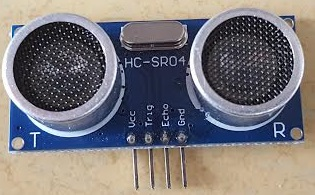
\includegraphics[scale=0.6]{DistanceMeasurementFront.jpg}
\centering
\caption{\it HC-SR04, avståndsmätaren i detta projekt.}
\end{figure} 


\noindent
Avståndsmätarens utdata fångas upp av en funktion. Denna konstrueras och kalibreras för att enligt målet bromsa in helt 1 cm från objektet. Kalibrering sker via testning av funktionen med olika inställningar där effektiviteten utvärderas. Utdatan från avståndsmätaren mäts även upp med hjälp av oscilloskop för att säkerställa att funktionen reagerar på rätt sätt vid olika värden.

\vspace{5mm} \noindent
Aktivering implementeras från två olika plattformar. Då både den sändande datorenheten och Androidapplikationen ska kunna initiera kontrollapplikationen konstrueras en möjlighet till detta på respektive system. %DETTA IMPLEMENTERAS MHA...


\newpage
\section{Teknisk beskrivning}
I denna sektion förklaras den tekniska delen av projektet. En bakgrund beskriver hur systemet fungerade ursprungligen. Detta följs av en översiktlig text över det ersättande systemet samt en sektion med mer detaljerande beskrivning över de separata delsystemen.


\subsection{Teknisk bakgrund}
För att kunna kontrollera en radiobil används en RF-sändare och en RF-mottagare ~\cite{RCTechnique}. Radiosignaler skickas från RF-sändaren och avkodas av RF-mottagaren i radiobilen, de kommunicerar över 2.4GHz-bandet. Dessa omvandlas då till elektroniska signaler som antingen kontrollerar bilens hastighet eller riktning. Parallellt med detta styrs även bilens hastighet, framåt eller bakåt, av motorns kraftutslag, medan riktningen beror på hjulens gradförskjutning. Bilens styrenhet omvandlar radiosignaler som sedan kontrollerar bilens rörelse.

\subsubsection{Styrsignaler}
Bilens styrsignaler kontrolleras av en kontrollenhet, MRX-242~\cite{projektDir}. Enheten fungerar simultant som radiomottagare och styrsignalsgenerator. Den genererar signaler till båda motorerna i bilen via tre kablar. I mening att replikera dessa finns även tillgång till ett ytterligare kopplingsblock.


\subsection{Systemöversikt}
Systemet har två huvuddelar, en MD407-enhet samt en Androidapplikation som båda kan agera handkontroll, och en MD407-enhet som genererar signaler till motorerna.

\subsubsection{Styrning: Från MD407 till MD407}
\begin{figure}[H]
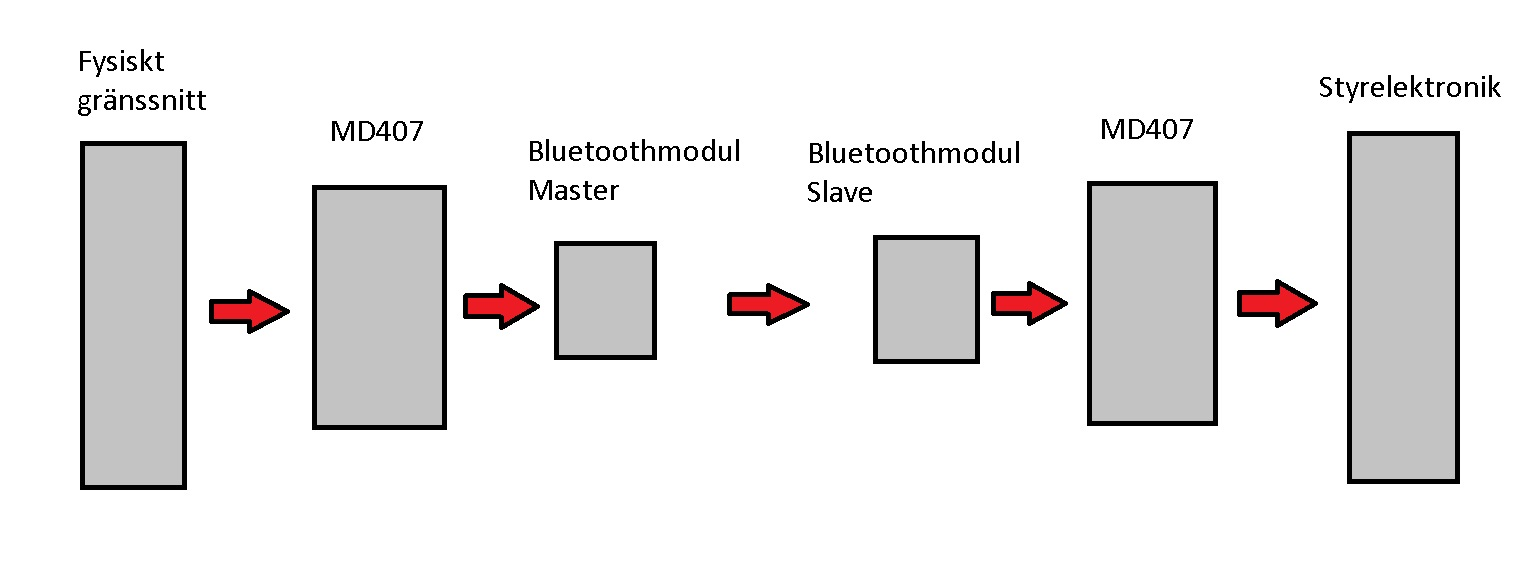
\includegraphics[width=\textwidth]{systemoversikt.jpg}
\centering
\caption{\it En översikt över systemet i blockformat med MD407 till MD407. Pilarna indikerar flödet av information, analogt eller digitalt.}
\end{figure} 


Enligt Figur 6 erhålls en överblick över hur systemet fungerar. Den sändande datorenheten MD407 får information från en potentiometer och skickar dessa värden via Bluetooth till den mottagande MD407-enheten som tar emot värdena och överlämnar dessa till bilens styrelektronik som agerar efter dem.

\subsubsection{Styrning: Från Androidapplikation till MD407}
\begin{figure}[H]
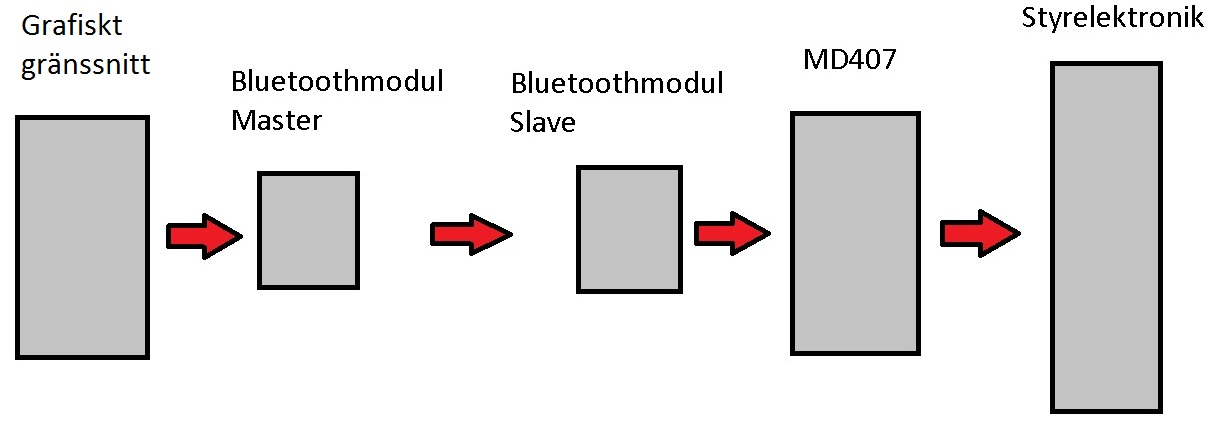
\includegraphics[width=\textwidth]{systemoversiktAndroid.jpg}
\centering
\caption{\it En översikt över systemet i blockformat med Androidapplikation till MD407. Pilarna indikerar flödet av information, analogt eller digitalt.}
\end{figure} 

Figur 7 visar en sammanfattning över systemet med en applikation som sändare. Observera att skillnaden mellan den tidigare styrningen är att Androidapplikationen skickar bytes genom sin integrerade Bluetooth-modul till mottagarens inkopplade. På samma sätt som tidigare analyseras sedan värdena och skickas till elektroniken i bilen.


\subsection{Delsystem}
Denna del av texten beskriver detaljerat hur de separata systemen fungerar. Ordningen baseras på flödet av information från sändare till mottagare och fram till bilens styrelektronik.




\subsubsection{Sändare: MD407-enhet}
Den sändande datorenheten MD407 skickar värden från potentiometern till den mottagande enheten. Sändaren försörjer dess inkopplade potentiometer med ström och läser konstant av utmatningsportarna för denna. På datorenheten finns en integrerad ADC, vilken tar emot värdena från potentiometern och översätter dessa från analoga till digitala värden. Det 8-bitars värde som skickas mellan sändare och mottagare (se Figur XX) ställs in enligt specifikationer. Ändras exempelvis vridkontakten på potentiometern för motorn ska kommandot initieras till det värde där mottagaren i sin tur sänder informationen till motorns elektronik. De 6 minst signifikanta bitarna beror på värdet datorenheten erhåller från potentiometern och tillsammans med kommandot skickas det seriellt från sändarens Bluetooth-modul och avläses i mottagarens.


\begin{figure}[H]
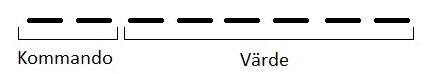
\includegraphics[scale=1]{aByteComVal.jpg}
\centering
\caption{\it Specifikationer av byten som seriellt skickas från sändare till mottagare.}
\end{figure} 




%Potentiometern kopplas enligt anvisningar från Figur 4 och även sedan till MD407 via en flatkabel för strömförsörjning enligt tidigare nämnd figur. Kablarna som kopplas till datorenheten sätts på PC1-porten och PC2-porten på MD407 i angiven ordning från figuren. De reglerar hastigheten respektive rattutslaget. Initiering av detta skrivs i C med utvecklingsmiljön Codelite.

%De tre kolumnerna av pinnar som finns i mitten på potentiometern(se Figur 2) använts till olika ändamål. Den mittersta kolumnen möjliggör för ström, därav får de vridbara kontakterna på potentiometern ström genom de korta sladdarna mellan strömkolumen till respektive vridkontakt. Sladden från den sista kolumnen på samma rad kopplat till MD407 ger värden konstant till datorenheten. På denna enhet finns en integrerad ADC. Denna tar emot värdena från portarna PC1 samt PC2 och översätter det till digitala värden. Genom RF-moduler kan de nya datorenheterna kommunicera. Resultatet skickas från sändarens RF-modul en byte åt gången 100 gånger i sekunden till mottagarens RF-modul. Specifikationerna som följs är att de första 2 bitarna indikerar kommandot och de resterande 6 bitarna med vilket värde kommandot ska utföras. 



\subsubsection{Sändare: Androidapplikation}
Androidapplikationen agerar som handkontroll. Detta följer samma protokoll som tidigare nämnts där de 2 mest signifikanta bitarna i varje byte bestämmer vilken sorts signal som ska ändras och de resterande bitarna bestämmer med vilket värde detta ska ske. Mobilapplikationen har på skärmen virtuella reglage (se Figur XX) som ska emulera ordinarie handkontrollens analoga funktion så att exempelvis hastighetsövergången är så jämn som möjligt. Denna skickar bytes seriellt till bilens dator via sin integrerade Bluetooth-modul.

\begin{figure}[H]
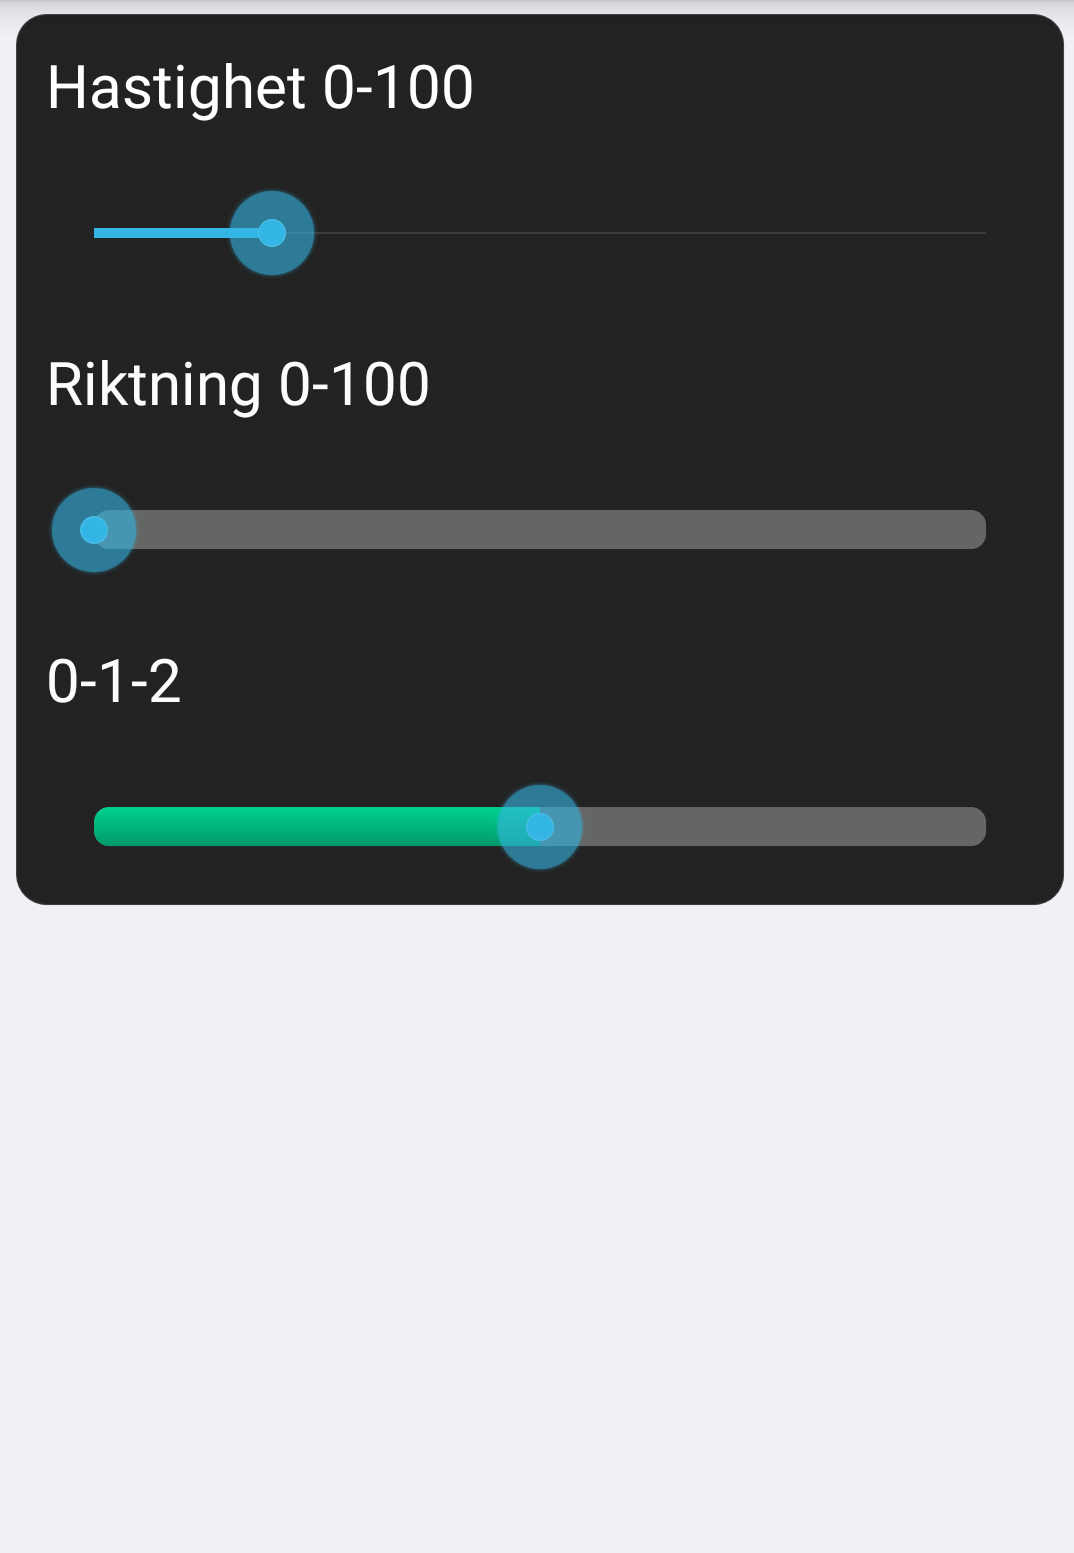
\includegraphics[scale=0.2]{applikation1.png}
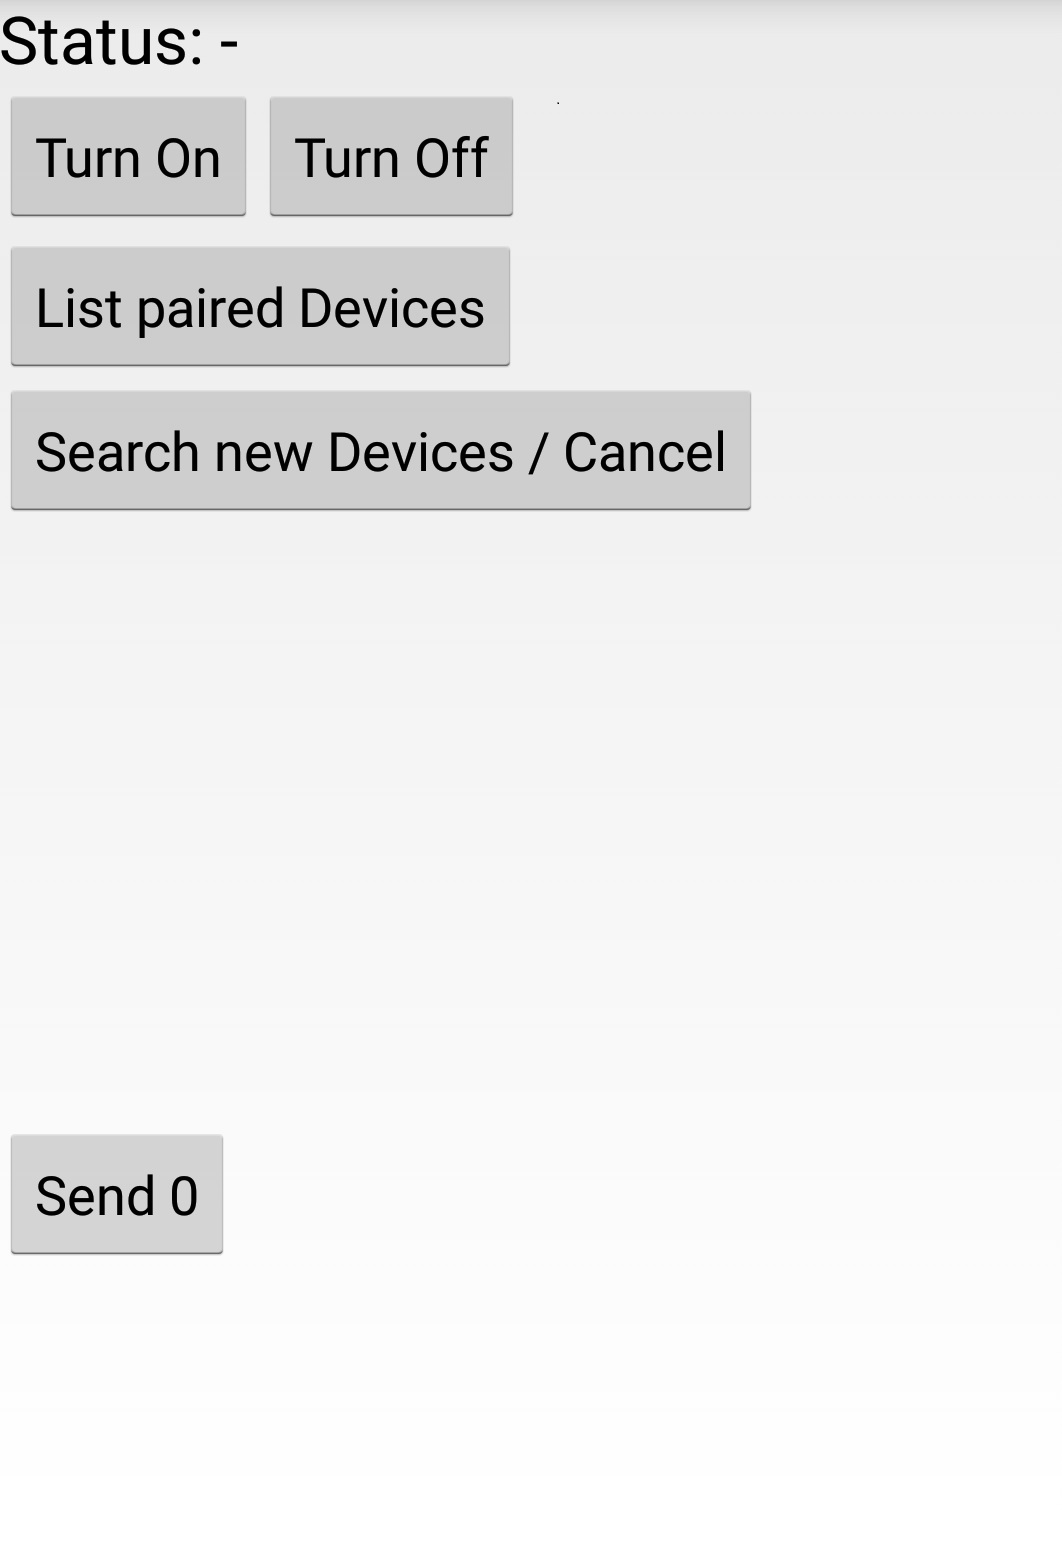
\includegraphics[scale=0.2]{applikation2.png}
\centering
\caption{\it Applikationens virtuella reglage (höger) samt applikationens Bluetooth-gränssnitt (vänster).}
\end{figure} 

\subsubsection{Kontrollapplikation}
Kontrollapplikationen kan aktiveras från en sändande enhet. Både MD407-enheten som agerar sändare och Androidapplikationen har en möjlighet att starta denna. %HUR


\vspace{5mm} \noindent
En $10\mu s$ hög puls triggar igång avstådsmätaren. Då detta sker får porten för eko på avståndsmätaren värdet 1 och ultraljud skickas ut. Om ultraljudet återvänder sätts eko-porten till 0 och pulsens bredd används för att bestämma avståndet till objektet. Detta sker genom att funktionen för kontrollapplikationen inkrementerar en variabel efter varje $\mu s$. Detta tal dividerat med 58 ger avståndet till hindret i cm~\cite{DistMeasure}. Ifall inget hinder uppmäts sänks pinnens värde till 0 efter en stund, pulsens längd tydliggör då att inget hinder finns i närheten.


Funktionen som styr kontrollapplikationen implementeras i mottagaren. Vid aktivering skickas värdet 155 till motorn  och bilen fortsätter köra i den hastigheten tills variabeln som mäter $\mu s$ uppnår värdet 8000, alternativt ungefär 138 cm, då värdet till motorn sänks till 151. Denna hastighet pågår tills bilen befinner sig 950$\mu s$ ifrån hindret, då den påbörjar motorbroms.


\subsubsection{Radiolänk: Bluetooth-modul}
Det som möjliggör kommunikation mellan sändare och mottagare är en Bluetooth-modul. Två likadana moduler kopplas till respektive datorenhet vilka då kan sända samt ta emot data från denna. Modulerna är antingen konfigurerade till att vara Master eller Slave. Master-modulen letar aktivt efter en Slave-modul i närheten och kommer vid upptäckt elektroniskt kopplas till den. Detta leder till att Master kan skicka data till Slave utan att riskera störningar från andra signaler.


\subsubsection{Mottagare: MD407-enhet}
Signalerna som sändaren skickar hanteras av mottagarens datorenhet. När programmet på denna dator påbörjas måste datorn initialt skicka PWM-signaler som motsvarar neutralt läge för drivmotorn i en kort stund innan övriga signaler kan sändas. Efter detta börjar mottagaren seriellt ta emot bytes från sändaren genom sin Bluetooth-mottagare. Enheten startar även PWM-signalsgenerering till bilens styrelektronik. 

\vspace{5mm} \noindent
Varje mottagen byte analyseras i mening att skicka en PWM-signal till korrekt elektronik i bilen. Som tidigare nämnt indikerar de 2 mest signifikanta bitarna till vilken del i styrelektroniken de resterande 6 bitarnas värde ska till. De 6 minst signifikanta bitarna kommer ha ett värde mellan 0-63 när mottagaren får dem. Till detta adderas en offset på 110 vilket gör att värdet istället befinner sig i intervallet 110-173. Syftar kommandot exempelvis på motorn (se Figur XX) kommer bilen åka i högsta möjliga hastighet bakåt vid värdet 110. Farten minskar sen vid högre värden och bilen når neutralt läge vid 142. Värden över detta upp till 173 får bilen att öka farten. Detta skickas sedan som PWM-signal till bilens styrelektronik som agerar med korrekt funktionalitet. Uppfattar bilen värden utanför detta intervall kan en överbelastning av bilens elektronik ske. 



%Utöver detta kan en kontrollapplikation påbörjas(FORTSÄTT VID MER INFO). 

\begin{figure}[H]
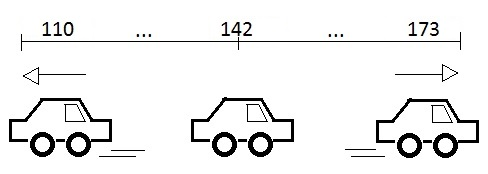
\includegraphics[scale=1]{110-173Car.jpg}
\centering
%SE ÖVER CAPTION, DENNA TEXT ÄR NÄMND I TEXTEN OVAN, ONDIG DÅ KANSKE
\caption{\it Illustrering av värdens effekter på bilen.}
\end{figure} 



%Datorn i bilen tar då emot ett kommandokod från Bluetooth-länken och analyserar detta i mening att specificera vilket kommando de två bitarna syftar på ska utföras. PWM-signalerna ändras sedan efter värdet på kommandot, de sex minst signifikanta bitarna, eller påbörjar kontrollapplikationen för demonstration. Motorerna tar emot PWM-signalerna och ger utslag beroende på deras medelspänning.

\subsubsection{Styrsignaler}
%Bilen uppfattar PWM-signaler 72 gånger i sekunden. De ursprungliga signalerna skickas på en frekvens av 72Hz, i mening att replikera dessa ges TIM2s räknare en frekvens av 100kHz. Ett antal klockcykler divideras med denna frekvens och kvoten ska då hamna nära 1/72. Antalet klockcykler är således bestämda till 1388. Resultatet av detta är att de nya PWM-signalerna skickas 72 gånger i sekunden till bilen som styrelektroniken läser av.

Bilens styrelektronik erhåller PWM-signaler från mottagaren. Under en period av klockcykler skickas delvis maximal spänning och delvis ingen spänning alls. Det antal klockcykler som skickar maximal spänning motsvarar det värde mottagaren erhållt från sändaren. Det som styrelektroniken då svarar på är hur stor andel av perioden som hög spänning mäts upp (se exempel i Figur XX). Denna procentenhet motsvarar en medelspänning som bilens styrelektronik direkt reagerar på. Intervallet som elektroniken i detta projekt svarar på är en andel på ungefär 8\%-12.4\%, alternativt en medelspänning på 269mV-423mV. Det förstnämnda värdet ger den maximala vänsterlutningen eller den högsta hastigheten bakåt beroende på vilket kommando som informationen från sändaren syftar på. Bilen kommer istället nå sin maximala högerlutning respektive högsta hastighet framåt om värdet är det sistnämnda. Intervallets mittersta värde ger ett neutralt läge i båda fallen.


\begin{figure}[H]
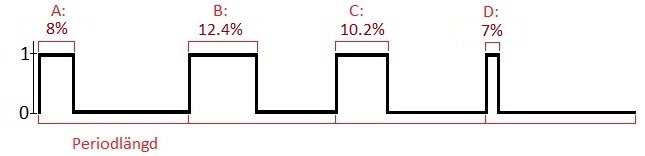
\includegraphics[scale=1]{PWMsignals.jpg}
\centering
\caption{\it Exempel på möjliga PWM-signaler. Om kommandot indikerar motorpåverkning kommer den i fall A och B köra i högsta fart baklänges respektive framlänges. I fall C hamnar bilen i neutralt läge och står då stilla. Signalen i fall D tolkas ej korrekt av bilens styrelektronik då det ligger utanför dess avläsningsintervall.}
\end{figure} 

%\vspace{5mm} \noindent
%PWM-signalerna kan endast avläsas korrekt av styrelektroniken på specifika värden. I varje period under en PWM-signal kan spänningen antingen vara 0, låg, eller 1, hög. Det som bilens styrelektronik svarar på är hur stor del av perioden signalen är hög (se Figur 3),  alternativt hur stor del av signalen som sänder 3.4V. Medelspänningen vid styrning och hastighet när styrningen är maximalt åt vänster respektive höger och hastigheten är maximalt bakåt respektive framåt går från 269mV till 423mV. Bilen når således högsta möjliga vänsterlutning samt fart bakåt vid 269mV, neutralt läge vid 348mV och maximal högerlutning samt fart framåt vid 423mV. Genom att dividera dessa värden enskilt med den maximala spänningen, som kan skickas från pinnarna på MD407, och sedan multiplicera med perioden, erhålls det värde bilens styrelektronik läser av. Detta resulterar i att bilen lyssnar på värden mellan 110-173 klockcykler under en period av 1388 klockcykler, det vill säga en andel av ungefär 8\%-12.4\% av hög signal. Detta styrs i bilen med hjälp av datorenhetens tidsmekanismer och dess standardbibliotek.

%\vspace{5mm} \noindent
%Information tas emot genom en mottagande modul. När mottagarmodulen erhåller ett meddelande triggas en funktion i koden. Denna ska undersöka vilket kommando som ska utföras samt till vilken grad detta skall göras enligt bitarnas anvisningar i Figur 2. Värdet 1 eller 2 på kommandobitarna leder till att bilens motor eller styrservo påverkas i angiven ordning. Tar mottagaren exempelvis emot kommandot att bilen ska ändra motorhastigheten skickas denna information till motorns styrelektronik. Den nya hastigheten beror på storleken av värdet. Värdet på meddelandet från sändaren skickas som en PWM-signal till den begärda styrelektroniken i bilen som fångar upp dessa under en period(se exempel i Figur 3), uppfattar värdet och agerar. Detta arbete har förenklats med hjälp av kodbibliotek från STMicroelectronics som innehåller funktioner för att initiera PWM-genererande. Observera att bilen endast svarar korrekt på värden där PWM-signalen är hög under ungefär 8\%-12.4\% av perioden, en högre eller lägre andel än detta kan få elektroniken att överbelastas. Värden i meddelanden mellan RF-modulerna kan antas från 0-63, utifrån 6 bitar, och TIM2 konfigureras därför till att addera en offset av 110 innan PWM-signalen skickas till styrelektroniken för att möjliggöra för korrekt avläsning.





\newpage
\section{Resultat}
Den resulterande produkten har under projektets tid nått verifikationspunkter. Dessa finns beskrivna nedan och även om de uppnåtts eller ej. För att kunna fastställa hur bra det ersättande systemet fungerar jämförs signalerna till bilen kontinuerligt så att det hela tiden skickas identiska signaler som i det ursprungliga systemet. Efter detta anges resultatet av hur väl projektplanen följts.

%Verifikationspunkter anges nedan och resultatet beskrivs efteråt.

\subsection{Sändare: MD407-enhet}
Den sändande datorenheten MD407 verifieras på följande punkter:
\begin{itemize}
\item Potentiometerns signal skickar rätt värden.
\item Md407-enhetens ADC ger digitala värden i korrekt intervall.
\item Kontrollapplikationen startas och utförs när detta begärs.
\end{itemize}

\noindent
Resultatet av detta är ett fullt fungerande system. Datorenheten får värden från potentiometern och dessa översätts korrekt till digitala värden som sedan kan skickas från sändaren.


\subsection{Sändare: Androidapplikation}
Följande punkter har verifierat att Andriodapplikationen fungerar enligt specifikation:

\begin{itemize}
\item Kan skicka värden till den mottagande enheten som ger korrekt följd.
\item Kontrollapplikationen startas och utförs när detta begärs.
\end{itemize}

%RESULTAT



\subsection{Mottagare: MD407-enhet}
Den mottagande MD407-enheten har verifierats enligt följande punkter:

\begin{itemize}
\item Kan ta emot värden från sändande enhet.
\item Skickar rätt PWM-signal till styrelektronik.
\item Har den ursprungliga bilens funktionaliteter.
\end{itemize}

\noindent
Genom projektet har styrsignaler konstant mätts upp. PWM-signalerna till styrelektroniken i bilen har under varje tillfälle mätts upp med hjälp av oscilloskop. Detta för att kunna urskilja vilka signaler bilen uppfattar, samt verifiera att värdena är korrekta.

\vspace{5mm} \noindent
Resultatet är ett fungerande system. Värden tas emot till den ottagande enheten via inkopplad mottagar-modul. Enligt oscilloskop ses att värdena till bilens styrelektronik är korrekta. Samtliga möjliga funktioner i det ursprungliga systemet har verifierats och fungerar som tidigare. Det vill säga hastigheten framåt och bakåt samt rattutslagen åt vänster och höger har testats korrekta.


\subsection{Radiolänk}
Informationsflödet mellan datorenheterna har testats i tre nivåer kontinuerligt under projektets gång:
\begin{itemize}
\item Kommunikation är möjligt via direktkopplad kabel.
\item Information kan sändas via RF-moduler.
\item Sändaren kan skicka information till mottagaren via Bluetooth.
\end{itemize}

\noindent
Vid slutfört projekt kunde alla punkter uppfyllas. Bilens ersättande mottagare kan kommunicera med sändaren via en direktkopplad kabel, en RF-modul och till slut en Bluetooth-modul. Under projektet har alla dessa tre steg följts upp för att ständigt veta att de fortfarande fungerar korrekt. När något ej fungerat i flödet mellan sändare och respons på styrsignal har kommunikationen gått ner en nivå för att lättare kunna felsöka.

\subsection{Kontrollapplikation}
Nedanstående punkter användes för att testa kontrollapplikationen.

\begin{itemize}
\item Stannar enligt specifikationer maximalt 1 cm från ett hinder vid maximala hastighet.
\item Fungerar från sändande MD407-enhet.
\item Fungerar från sändande Andriodapplikation.
\end{itemize}

%RESULTAT


\subsection{Verifikation av projektplan}
Mindre förändringar har under projektets gång skett. Då ersättandet av kontrollen samt mottagaren varit mer komplicerade än projektgruppen tidigare trott tog denna procedur 3 veckor längre tid än väntat. Detta problem har troligtvis försämrat kvalitén på kontrollapplikationen men ej Androidapplikationen då denna konstruerats parallellt med det nya systemet.



\newpage
\section{Diskussion och Slutsats}
%TA MED ATT DET TOG LÄNGRE TID BC FEL I BIBLIOTEK, STYRSERVO SÖNDER

%VARFÖR MÅL 1 TOG LÄNGRE TID
Projektet följde ej tidsmodellen som givits i planen. Ett antal felskrivanden i de tillhandahållna biblioteken ledde till extra verifikation för att kunna erhålla rätt hjälpfunktioner. Utöver detta gick bilens styrservo sönder på grund av felaktiga PWM-signaler som överbelastat systemet. Arbetet krävde därav lite mer tid när detta skedde. I det stora hela var implementationen av de ersättande mottagar- och sändarnodarna mer invecklade än vad som uppfattats vid början av projektet och detta ledde i sin tur till tid som gick till extra verifikation. Parallellt arbete utnyttjades dock, vilket gjorde att produkten trots allt blev färdig som planerat.

%HUR VI BESTÄMDE SPECIFIKATIONER ÖVER KONTROLLAPPLIKATION
\vspace{5mm} \noindent
Kontrollapplikationen kunde ej färdigställas som tänkt. Målet var att bilen efter aktivering av applikationen skulle stanna maximalt 1 cm från närmaste hinder, men detta har ej kunnat implementeras under den givna tiden. Detta beror dels på att avståndsmätaren är av en enklare variant och då inte alltid ger pålitliga värden. Dels på att hjulen inte alltid är raka vilket på en längre sträcka gör att bilen hamnar i ett snett läge. Resultatet blir då att ultraljudet avståndsmätaren skickar ut riskerar att studsa snett. Detta kan i sin tur leda till att ultraljudet tas upp vid felpunkt eller inte alls, vilket ger felberäkningar. Utöver detta har bilens bromsfunktion försvårat arbetet. Bilens egna funktion för motorbromsning resulterar inte till att bilen stannar tvärt, snarare att den rullar sakta innan den helt står stilla. Även i neutralt läge kan hjulen rotera lite ifall däcken står på en dubb. Däcken roterar då tills den är mellan två dubbar. Detta ledde till att det blir osannolikt att ha två likadana fall då bilens bromssträcka beror från test till test. Att då bestämma en konstant funktion som ska fungera för samtliga fall blir väldigt komplicerad. 


\vspace{5mm} \noindent
Ett par faktorer hade kunnat förbättra kontrollapplikationen om mer tid funnits. Till att börja med hade en bättre avståndsmätare givit bättre värden. Värdesfel som den enklare modellen ger ibland hade då undvikts. Dessutom hade fler avståndsmätare lett till bättre verifiering för bilens omkringliggande miljö. Försämringar av kontrollapplikationen då bilens hjul är något svängda hade kunnat reduceras radikalt om inte helt elimineras.


%Kontrollapplikationen kunde ej färdigställas som tänkt. Planen var att när bilen uppnåt sin maximala hastighet skulle applikationen aktiveras och bilen skulle vid första hinder stanna 1 cm från det. Vid en första verifiering upptäcktes det dock att detta skulle bli för komplicerat med de hjälpmedel som fanns tillgängliga. För det första vibrerar bilen kraftigare ju högre hasstgighet den har. Detta leder till att ultraljudet avståndsmätaren skickar iväg inte alltid återvänder, då det missas om bilen är i en annan höjd. Något som sker vid vibrationer. För det andra skulle det behövas en bättre, alternativt fler, avståndsmätare. Detta skulle resultera i bättre och snabbare beräkning av avstånd till närmaste hinder och på så sätt börja bromsa bilen vid rätt läge. Den mätaren som givits i detta projekt når inte upp till dessa kvalifikationer och behöver därför en lägre hastighet för att garantera kontrollapplikationens funktion, därav garantera bilens säkerhet.











%HÄR BÖRJAR FÖRSLAG PÅ VIDARE FORSKNING/UPPGRADERING

%HANDKONTROLL
\vspace{5mm} \noindent
Projektgruppen vill belysa en möjlig designuppgradering till handkontrollen. Delsystemen är implementerade endast genom hårdvara, ett konsumentvänligt lager finns ej. Detta möjliggör då för enorma designmöjligheter för en butiksfärdig produkt. Då bilens styrelektronik vid felaktiga PWM-signaler kan överbelastas anser projektgruppen att en maximal och minimal vridbarhet på potentiometern borde finnas. Detta är något som skulle kunna implementeras samtidigt som ett användarvänligt skal för handkontrollen konstrueras.


%ANDROIDAPPLIKATION
\vspace{5mm} \noindent
Med Androidapplikationen ses stora möjligheter. 2013 ägdes en smartphone av ungefär 90\% av Sveriges befolkning mellan 12-45 år~\cite{smartphoneStat}. Telefonapplikationen vänder sig till en väldigt stor andel av folket och projektgruppen ser därför positivt på att utveckla denna. Fokuset med Androidapplikationen har varit på en hårdvarunivå och utseendet är därför inte så tilltalande. Potentialen för att vidareutveckla applikationen är således väldigt god och det blir då möjligt att fokusera på designen och implementation över flertal operativsystem. Med tanke på andelen människor som skulle kunna använda denna telefonapplikation anser projektgruppen att den väger tungt för marknaden. En konsument som innehar applikationen skulle kunna koppla sin telefon via Bluetooth till sin radiobil och handkontrollen blir då inte längre en extra komponent som behöver bäras med. Samma konsument skulle även kunna styra andra radiobilar rent intuitivt, så länge denna bil har en mottagande Bluetooth-modul och likadana kommandofunktioner. Skulle detta möjliggöras kan det behövas att konstruera ett säkerhetslager så att oinbjudna parter ej kan styra bilen.

%KONTROLLAPPLIKATION
\vspace{5mm} \noindent
Om man ser till ett större perspektiv finns även här implementationsförslag. Kontrollapplikationen skulle i framtiden kunna spela en stor roll. Även fast koden som använts i det här projektet endast fungerar med samma moduler som utnyttjats, hindrar inte det användning i större sammanhang. Det aktuella forskningsområdet, självstyrande bilar, har gjort att många frågor kring säkerhet ställts. En kontrollapplikation som vid aktivering stannar på ett visst maximalavstånd från ett hinder skulle kunna spela stor roll i passagerarnas säkerhet. Detta skulle då behöva fler, större sensorer och koden skulle behöva använda sig av mer verifierade funktioner för att kunna garantera säkerhet.  



%En radiobil är bara ett exempel på produkter där projektets mål kan appliceras. Andra produkter som styrs via radiolänk kan även de uppdateras enligt denna projekts modell. 

%Tekniken är färdigställd, överförandet till en konsumentvänlig produkt 



\vspace{5mm} \noindent
%SAMMANFATTNING, GLÖM INTE ATT ÅTERKOPPLA TILL INLEDNING
Sammanfattningsvis innehåller detta projekt en radiostyrd bil med modern teknik. Uppgradering med nya datorer reducerar utdaterad teknik och dess funktioner passar väl in med det som idag är aktuellt. Potentialen för vidareutveckling hos handkontrollen samt Androidapplikationen är väldigt god. Utöver detta finns även stora designmöjligheter för att konstruera komponenterna till mer konsumentvänliga produkter. I det större perspektivet finns idag smartphones hos en ännu större del av befolkningen än tidigare nämnt, vilket resulterar i en ännu större potentiell marknad för telefonapplikationen. Dagens teknik fokuserar även mycket på självstyrande bilar och en funktion som undviker krock kan komma att spela stor roll. Både för passagerarnas säkerhet, men även miljön runt omkring bilen där demolering undviks. Kort sagt öppnar detta projekt upp för en nyskapande radiostyrd bil där aktuell teknologi är implementerad och bilens funktioner kan i ett makroperspektiv användas till många olika ändamål.





\newpage
%To references
\addcontentsline{toc}{section}{Bibliography}\bibliographystyle{IEEEtran}
\bibliography{referenserRapport}


\end{document}

